%% ****** Start of file apstemplate.tex ****** %
%%
%%
%%   This file is part of the APS files in the REVTeX 4.2 distribution.
%%   Version 4.2a of REVTeX, January 2015
%%
%%
%%   Copyright (c) 2015 The American Physical Society.
%%
%%   See the REVTeX 4 README file for restrictions and more information.
%%
%
% This is a template for producing manuscripts for use with REVTEX 4.2
% Copy this file to another name and then work on that file.
% That way, you always have this original template file to use.
%
% Group addresses by affiliation; use superscriptaddress for long
% author lists, or if there are many overlapping affiliations.
% For Phys. Rev. appearance, change preprint to twocolumn.
% Choose pra, prb, prc, prd, pre, prl, prstab, prstper, or rmp for journal
%  Add 'draft' option to mark overfull boxes with black boxes
%  Add 'showkeys' option to make keywords appear
%\documentclass[aps,prl,preprint,groupedaddress,showkeys]{revtex4-2}
%\documentclass[aps,prl,preprint,superscriptaddress,showkeys]{revtex4-2}
\documentclass[aps,prfluids,reprint,nofootinbib,onecolumn,groupedaddress,showkeys]{revtex4-2}


\usepackage{amssymb}
\usepackage{amsmath}
\usepackage{mathptmx,mathtools}
\usepackage{array}

\usepackage[export]{adjustbox}
\usepackage{array} 
\newcolumntype{C}[1]{>{\centering\arraybackslash}m{#1}} % centered + vertical middle
\usepackage[percent]{overpic}
\usepackage[caption=false]{subfig}
\usepackage{amsmath}
\usepackage{nicefrac}
\usepackage{dirtytalk}
\usepackage{graphicx}
\usepackage{tikz} 
\usepackage{xcolor}
\usepackage{lineno}
%\bibliographystyle{apsrev4-2}
\renewcommand\linenumberfont{\normalfont\small} % <-- Increase line number size
\renewcommand{\thetable}{\Roman{table}}

% ---- in your preamble ----
\usepackage{array} % needed for m{}, p{}, \arraybackslash
\newcolumntype{M}[1]{>{\centering\arraybackslash}m{#1}} % centered fixed-width col
\renewcommand{\arraystretch}{1.15} % (optional) taller rows


\begin{document}
	
	\linenumbers
	
	%Title of paper
	\title{Dynamics of a Rising Bubble from a Lagrangian Coherent Structures Perspective}
	
	\author{Behnam Kazemi Majd}
	\thanks{Contact author: behnam.k.majd@ntnu.no}
	\author{Rohith Jayaram}
	\author{Sanjid S. Chirammel}
	\author{Jannike Solsvik}
	
	\affiliation{Department of Chemical Engineering, Norwegian University of Science and Technology (NTNU), Trondheim, Norway}
	
	\date{\today}
	
	\begin{abstract}
		The wake of a rising bubble plays a central role in determining its rise behavior, shape deformation, and interaction with neighboring bubbles. However, conventional visualization methods such as streamlines or vorticity fields often fail to objectively identify the wake boundary and its transport characteristics. In this work, an objective, Lagrangian framework based on Lagrangian Coherent Structures (LCSs) is employed to characterize the wake of a single bubble rising in a quiescent liquid. The velocity fields are obtained from axisymmetric simulations using an in-house Sharp Interface Level-Set Method (SI-LSM$_\text{col}$). The analysis reveals that the innermost repelling LCS coincides with the physically observed wake boundary, providing a material, frame-invariant definition of wake length measured consistent with the experimental correlations. The identified structures effectively separate the flow into regions of distinct transport behavior, governing the entrainment of non-inertial particles into the recirculating zone. Furthermore, the backward finite-time Lyapunov exponent field from the leading-bubble flow qualitatively {\color{black}explains} the acceleration of a trailing bubble in coalescence scenarios, linking stronger attracting regions to enhanced velocity deficit. The results highlight the ability of LCSs to unify wake topology, tracer transport, and bubble interaction into a coherent physical description of multiphase flow problems is the(axisymmetric) multiphase flows.
	\end{abstract}
	
	\keywords{Rising bubble, wake, vortical structures, LCS, coalescence}
	
	\maketitle
	
	\section{Introduction}
	\label{Introduction}
	
	One of the well-known and classic multiphase-flow problems is a single bubble rising due to buoyancy in a quiescent fluid. There is a rich literature, from the early 1970s to the present, using both numerical simulations and experiments to investigate this problem. Researchers have focused on different dynamical aspects such as bubble-rise characteristics~\cite{clift1978}, the wake structure~\cite{Bhaga1981,Lozano2016}, and the transport and mixing of species~\cite{Calderbank1970,Brignell1974,Zun2012,siow2025}. Except in a few simplified models—for example, when viscous and inertial effects are negligible—most formulations yield incomplete or inaccurate descriptions of bubble dynamics if wake effects are not considered~\cite{Liang1990}. The wake can therefore be viewed as a unifying lens that links the observed behaviors of bubble rise, shape deformation, and path instability to the underlying wake dynamics. Moreover, the bubble wake is a driving mechanism for coalescence, bouncing, or evasion of two in-line rising bubbles~\cite{Liao2010}. In industrial applications involving rising bubbles, the wake is critically important for mass transfer~\cite{Jimenez2013}. These lines of evidence highlight the importance of the bubble wake that is comprehensively discussed in \cite{Liang1990} and \cite{clift1978}.
	
	Generally speaking, the wake of a bluff body exhibits complex and diverse shapes depending on the system dynamics and flow characteristics. For a rising bubble, a well-defined characterization of the wake exists in terms of the bubble Reynolds number and the Morton number of the system~\cite{clift1978}. The laminar wake is observed for $Re<110$ characterized by a pair of toroidal vortices, which remain stable in highly viscous flows with large Morton numbers. As the Reynolds number increases or the Morton number decreases, these vortices become unstable and start shedding due to instabilities in the rising dynamics~\cite{Coppus1977,Tripathi2015}. Following the dual-wake-structure concept in \citet{Liang1990}, the wake is divided into primary and secondary regions, with closed, quasi-stationary toroidal vortices that convect with the bubble in the former, and shear layers that extend downstream in the latter. 
	
	There have been both experimental and numerical works examining the properties of the primary wake and its critical role in in-line interactions between bubbles. From the comprehensive experimental visualizations of \citet{Bhaga1981,Bhaga1980Exp}, the wake geometry was characterized in terms of its overall length and width obtained from projected images. In particular, the laminar wake length was found to depend primarily on the Reynolds number for $\mathrm{Mo} > 4\times10^{-3}$. Moreover, they proposed a wake-velocity model derived from velocity measurements using the hydrogen-bubble tracer technique. Building on streamline patterns obtained from numerical simulations, \citet{Monica2016} proposed a predictive model relating the critical Reynolds number to the Eötvös number, below which toroidal vortices are not observed even when the bubble is deformed. Motivated by the critical role of the bubble wake in in-line bubble interactions~\cite{Yuan1994,HALLEZ2011,Gumulya2017}, numerous studies have investigated the governing mechanisms in bubble coalescence, either by employing wake-velocity models~\cite{Narayanan1974,Zhang2003,Ramirez2014} or by analyzing the flow structures~\cite{Brucker1999,Smolianski2005,Kusuno2021}. While their findings are of considerable value, they mostly rely on Eulerian visualizations such as vorticity fields, streamlines, or the Q-criterion~\cite{Senapati2019,Zhao2024}. These techniques often limit the understanding of the wake to its geometry and configuration and require consideration of additional field variables to analyze the role of flow structures in mixing and transport. Another limitation is the lack of objectivity (frame dependence), which makes these identification methods unreliable for robust analysis, as they may yield different structures in different frames of reference. Therefore, a concise, mathematical, and objective description rooted in Lagrangian material coherence is required.
	
	An objective criterion was developed based on the Lagrangian coherence of material trajectories, which define flow structures known as Lagrangian Coherent Structures (LCSs)~\cite{Haller2015}. These structures are materially Lagrangian-coherent in the sense that they are advected with the flow while preserving their overall dynamics and functioning as effective transport barriers over a finite time interval. In the context of rising bubble, \citet{Ming2017} was the first to employ this relatively new technique to identify LCSs for examining transport phenomena around bubbles. \citet{Kameke2019} employed LCS analysis and revealed unexpectedly long residence times in the bubble wake. The most recent study is the experimental work of \citet{Kursula2022} where dissolved-gas concentration patterns and mixing were linked to the underlying flow structures. These recent studies indicate the versatility of the LCS in uncovering diverse flow phenomena and emphasize its growing potential as a relatively new approach for multiphase-flow analysis.
	
	Although many studies employ Lagrangian Coherent Structures (LCS) in the context of the rising bubble problem, to the best of our knowledge, an objective characterization of the wake structure has not yet been reported. Given the importance of such a description, we address this gap by adopting the LCSs to provide a material, frame-invariant description of the bubble wake boundary. Furthermore, the objective description of the wake enables an in-depth analysis of the particle motion above the bubble, demonstrating how the LCS regulate entrainment into the wake. In addition, the acceleration effect experienced by a trailing bubble rising within the wake of a leading bubble is qualitatively discussed. This provides an intuitive and physically consistent explanation of the acceleration effect {\color{black}in inline, axisymmetric} rises.
	
	The remainder of this paper is organized as follows. Section \ref{Numerical setup} describes the numerical formulation and the set of simulated cases used for the LCS analysis. Section \ref{Lagrangian Coherent Structures} outlines the theoretical background of LCSs and their computation from the velocity fields. The results and discussion are presented in Section \ref{Results and discussion}, where the objectivity of the method, the wake structure, tracer transport, and the coalescence mechanism are analyzed in detail. Finally, Section \ref{Concluding remarks} summarizes the main findings.
	
	\section{Numerical setup}
	\label{Numerical setup}
	\label{Mathematical formulation}
	This section briefly presents the numerical setup utilized by an in-house Computational multi-Fluid Dynamics solvers\textemdash Sharp Interface Level Set Method on Co-located grid (SI-LSM$_{\text{col}}$) \cite{Chirammel2023}. The velocity fields for LCS analysis are obtained from the solution of conservation equations using SI-LSM$_{\text{col}}$ on an \textit{axisymmetric} coordinate system. The SI-LSM$_{\text{col}}$ utilizes a \textit{sub-domain conservation law}-based formulation with interfacial jump boundary condition. Validation of these in-house solver and detailed discussion on the numerical methodology are presented elsewhere \cite{Chirammel2023}, whereas for clarity, the utilized non-dimensional conservation equations are given here as follows
	\subsection*{Continuity Equation:}
	\begin{equation}\label{eqt:continuity}
		\nabla\cdot\mathbf{U}=0
	\end{equation}
	\subsection*{Momentum equation:}
	\noindent For SI-LSM$_{\text{col}}$:
	\begin{equation}\label{eqt:momEqt-SI}
		\frac{\partial(\chi_{i}\mathbf{U})}{\partial\tau}+\nabla\cdot(\chi_{i}\mathbf{U}\mathbf{U})=-\nabla P+\frac{1}{Ga}\nabla\cdot(\eta_{i}[\nabla\mathbf{U}+\nabla\mathbf{U}^T])-\frac{\chi_{i}}{Fr^2}\hat{j}
	\end{equation}
	
	\noindent where $\tau$, $\mathbf{U}$, $P$, $\kappa$, and $\hat{\mathbf{j}}$ denote the nondimensional time, velocity vector, pressure, interface curvature, and the unit vector along the $z$-axis in an \textit{axisymmetric} coordinate system, respectively. The equations are nondimensionalized using the bubble diameter $D$ as the length scale, gravitational acceleration $g$, the velocity scale $u_c=\sqrt{gD}$, and the time scale $t_c=D/u_c$, which yields $Fr=1$. Using these scales, the nondimensional variables are given by:
	\begin{equation*}
		\mathbf{X}=\frac{\mathbf{x}}{D}; \mathbf{U}=\frac{\mathbf{u}}{u_c}; \tau=\frac{t}{t_c}; P=\frac{p}{\rho_1u_c^2}
	\end{equation*}
	and the corresponding non-dimensional numbers are
	\begin{equation*}
		Re = \frac{\rho_1 U_T D}{\mu_1};~~ Ga=\frac{\rho_1 D \sqrt{gD}}{\mu_1};~~ Eo=\frac{\rho_1g D^2}{\sigma};~~ Mo = \frac{Eo^3}{Ga^4} \ 
	\end{equation*}
	where $Re$ (inertia-to-viscous), $Eo$ (buoyancy-to-surface tension), $Ga$ (buoyancy-driven inertia to viscous damping, velocity-free), and $Mo$ (fluid-property group), respectively. Here, $\rho$, $\mu$, and $\sigma$ are the density, dynamic viscosity, and surface tension, respectively. 
	
	%%%%%%%%%%%%%%%%%%%%%%%%%%%%%%%%%%%%%%%%%%%%%%%%%%%%%%%%%%%%%%%%%%%%%%%%%%%%%%%%%
	%%%%%%%%%%%%%%%%%%%%%%%%%%%%%%%%%%%%%%%%%%%%%%%%%%%%%%%%%%%%%%%%%%%%%%%%%%%%%%%%%
	%%%%%%%%%%%%%%%%%%%%%%%%%%%%%%%%%%%%%%%%%%%%%%%%%%%%%%%%%%%%%%%%%%%%%%%%%%%%%%%%%
	%%%%%%%%%%%%%%%%%%%%%%%%%%%%%%%%%%%%%%%%%%%%%%%%%%%%%%%%%%%%%%%%%%%%%%%%%%%%%%%%%
	%%%%%%%%%%%%%%%%%%%%%%%%%%%%%%%%%%%%%%%%%%%%%%%%%%%%%%%%%%%%%%%%%%%%%%%%%%%%%%%%%
	%%%%%%%%%%%%%%%%%%%%%%%%%%%%%%%%%%%%%%%%%%%%%%%%%%%%%%%%%%%%%%%%%%%%%%%%%%%%%%%%%
	%%%%%%%%%%%%%%%%%%%%%%%%%%%%%________Figure_1___________%%%%%%%%%%%%%%%%%%%%%
	\begin{figure}[!t]
		\centering
		
\includegraphics[scale=0.8,trim={1.5cm 8.5cm 1.5cm 6cm},clip]{Figure_1.pdf}
		\caption{(a) Location of the simulated cases (C$_1$–C$_7$) from Table~\ref{Table1} on the Eötvös–Galilei (Eo–Ga) map for rising bubbles. The red dashed line indicates a constant Morton number (Mo = $10^{-3}$), while the blue dashed line divides break-up region from non-breaking region adopted from~\cite{Tripathi2015}. (b) Schematic of the two-dimensional \textit{axisymmetric} computational domain employed in the rising-bubble simulations using SI-LSM$_\text{col}$, including both single- and two-bubble configurations.}
		\label{Fig1}
	\end{figure}
	%%%%%%%%%%%%%%%%%%%%%%%%%%%%%________Figure_1_end___________%%%%%%%%%%%%%%%%%%%%%
	%%%%%%%%%%%%%%%%%%%%%%%%%%%%%%%%%%%%%%%%%%%%%%%%%%%%%%%%%%%%%%%%%%%%%%%%%%%%%%%%%
	%%%%%%%%%%%%%%%%%%%%%%%%%%%%%%%%%%%%%%%%%%%%%%%%%%%%%%%%%%%%%%%%%%%%%%%%%%%%%%%%%
	%%%%%%%%%%%%%%%%%%%%%%%%%%%%%%%%%%%%%%%%%%%%%%%%%%%%%%%%%%%%%%%%%%%%%%%%%%%%%%%%%
	%%%%%%%%%%%%%%%%%%%%%%%%%%%%%%%%%%%%%%%%%%%%%%%%%%%%%%%%%%%%%%%%%%%%%%%%%%%%%%%%%
	%%%%%%%%%%%%%%%%%%%%%%%%%%%%%%%%%%%%%%%%%%%%%%%%%%%%%%%%%%%%%%%%%%%%%%%%%%%%%%%%%
	
	Further, the non-dimensional physical properties of the fluids are defined as
	\newline
	\noindent For SI-LSM$_{\text{col}}$:  
	\begin{equation*}
		\begin{aligned}
			&\chi_{i}=H(\phi_{LSM}) + \chi H(\phi_{LSM})\\
			&\eta_{i}=H(\phi_{LSM}) + \eta H(\phi_{LSM})
		\end{aligned}
	\end{equation*}
	where
	\begin{equation*}
		\chi=\frac{\rho_2}{\rho_1}\text{ and }\eta=\frac{\mu_2}{\mu_1}
	\end{equation*}
	and
	\begin{equation}\label{eqt:heaviside_SI}
		H(\phi_{LSM})=\begin{cases}
			1&\phi_{LSM}\ge0\\
			0&\phi_{LSM}< 0
		\end{cases}
	\end{equation}
	\newline
	
	
	where $\phi_{LSM}$ is the level-set function representing two fluids with positive and negative values with the $\phi_{LSM}=0$ contour corresponds to the interface separating the two fluids. 
	
	For the present SI, the momentum equation is solved along with an interfacial jump boundary condition, given as 
	\begin{equation}\label{eqt:Pressure_JumpBC}
		[P]= P_{1,\Gamma}-P_{2,\Gamma}=\frac{\kappa}{We}+\frac{2}{Re}(\eta_{1}-\eta_{2})\hat{N}\cdot(\nabla U\cdot\hat{N},\nabla V\cdot\hat{N})
	\end{equation}
	where the subscripts 1, 2, and $\Gamma$ correspond to fluid-1, fluid-2 and interface, respectively. Further, $\hat{N}$ is the unit normal and defined as 
	
	\begin{equation}\label{eqt:heaviside_SI2}
		\hat{N}=\frac{\nabla\phi_{LSM}}{|\nabla\phi_{LSM}|}
	\end{equation}
	
	\subsubsection*{Interface Advection Equation:}
	\noindent For SI-LSM$_{\text{col}}$:
	\begin{equation}\label{eqt:LSadvection}
		\frac{\partial\phi_{LSM}}{\partial\tau}+\mathbf{U}\cdot\nabla\phi_{LSM}=0
	\end{equation}
	
	Further for SI, the advected $\phi_{LSM}$ is reinitialized as a normal distance function by solving a reinitialization equation, given as
	\begin{equation}\label{eqt:reinitialization}
		\frac{\partial\phi_{LSM}}{\partial\tau_s}=S_{\epsilon}(\phi_{LSM,0})(1-|\nabla\phi_{LSM}|)
	\end{equation}
	where $\tau_s$ and $S_{\epsilon}$ denotes pseudo time step and smoothened sign function \cite{Sussman1994}, defined as
	\begin{equation*}
		\tau_s=\frac{\Delta X}{10} \text{ and } S_{\epsilon}=\sqrt{\frac{\phi_{LSM,0}}{\phi_{LSM,0}^2+\Delta X^2}}
	\end{equation*} 
	
	\noindent where $\phi_{LSM,0}$ corresponds to the $\phi_{LSM}$ value before pseudo iteration in Eq. (9). 
	
    %%%%%%%%%%%%%%%%%%%%%%%%%%%%%%%%%%%%%%%%%%%%%%%%%%%%%%
    %%%%%%%%%%%%%%%%%%%%%%%%%%%%%%%%%%%%%%%%%%%%%%%%%%%%%%
    %%%%%%%%%%%%%%%% Table 1 %%%%%%%%%%%%%%%%%%%%%%%%%%%%%
    %%%%%%%%%%%%%%%%%%%%%%%%%%%%%%%%%%%%%%%%%%%%%%%%%%%%%%
    \begin{table}[!tbp]
    \centering
    \caption{Non-dimensional parameters of the selected cases. All cases are solved on a grid size of $D/62.5$ with $\chi=0.01$ and $\eta=0.01$. (*Cases $C_4$ and $C_7$ are considered for coalescence of two bubbles.)}
    \vspace{0.3cm}
    \begin{tabular*}{\linewidth}{@{\extracolsep{\fill}} c c c c c }
    \hline\hline
    Case & Ga & Eo & Mo & Re \\
    \hline
    C$_1$  & 15   & 70  & $5.7$ & 6.4\\
    C$_2$  & 21   & 92  & $3.8$ & 10\\
    C$_3$  & 26   & 50  & $2.6\times10^{-1}$ & 13.4\\
    C$_4^*$  & 32 & 22   & $1.0\times10^{-2}$ & 18.3 \\
    C$_5$  & 35  & 115  & $1.02$ & 18.7\\
    C$_6$ & 72  & 24   & $5.17\times10^{-4}$ & 44\\
    C$_7^*$  & 97  & 98  & $1.0\times10^{-2}$ & 61 \\
    \hline\hline
    \end{tabular*}
    \label{Table1}
    \end{table}
    %%%%%%%%%%%%%%%%%%%%%%%%%%%%%%%%%%%%%%%%%%%%%%%%%%%%%%
    %%%%%%%%%%%%%%%%%%%%%%%%%%%%%%%%%%%%%%%%%%%%%%%%%%%%%%
    %%%%%%%%%%%%%%%% Table 1 end %%%%%%%%%%%%%%%%%%%%%%%%%
    %%%%%%%%%%%%%%%%%%%%%%%%%%%%%%%%%%%%%%%%%%%%%%%%%%%%%%


	Under the current numerical method on an axisymmetric coordinate system, bubbles with rectilinear rising paths and symmetric behavior can be simulated. This condition inherently restricts the analysis to cases with $\mathrm{Mo} > 1\times10^{-3}$ and $Ga<100$~\cite{Hua2007}. In addition, bubble breakup should be avoided, as it may introduce complex physical phenomena such as peripheral breakup or instability which are beyond the scope of this study. \citet{Tripathi2015} identified a Ga–Eo boundary below which bubbles remain stable and avoid breakup. Considering these restrictions, seven cases, listed in Table~\ref{Table1} and shown in the Eo–Ga map in Figure~\ref{Fig1}(a), are selected for analysis. These represent stable bubbles within the laminar regime, where the wake behavior is primarily governed by the Reynolds number. Hence, case $C_7$ with $\mathrm{Mo} = 1\times10^{-2}$ and $Ga = 97$ represents a comparatively high Reynolds number of 61 under the given conditions. This case serves as a reference for cases 1–6, where viscosity and bubble diameter are varied independently to obtain cases with different $\mathrm{Mo}$ and $\mathrm{Re}$ numbers, respectively. They are solved for the computational domain given in Figure~\ref{Fig1}(b) with the assumed boundary conditions.
	
	To analyze the effect of the Reynolds number on the wake and its influence on bubble coalescence, the size of the leading bubble is varied. Case $C_4$ with diameter $D_1$ is considered as the reference trailing-bubble case. The leading bubble is first assumed to have the same size $D_1$ (low-Reynolds-number case) and then compared with the larger-bubble case $C_7$, with diameter $D_2$ (high-Reynolds-number case). In this configuration, the leading bubble is released at a nondimensional axial position of $Z = 3D_2 / D_1$ from the bottom of the channel at $\tau_0$. It should be noted that, to analyze the effect of the separation distance on coalescence, the trailing bubble is released at $\tau_0 + \Delta \tau$ (delayed release), resulting in different nondimensional inter-spacing $S$ between the two bubbles. Here in this work, the inter-spacing $S$ is defined as the distance between the lower surface of the leading bubble and the roof of the trailing bubble as shown in Figure~\ref{Fig1}(b).
	
	%hi
	\section{Lagrangian Coherent Structures}
	\label{Lagrangian Coherent Structures}
	In this section the theoretical foundation of Lagrangian coherent structures are presented. In principal, Lagrangian trajectories of tracers can be used to reveal the temporal evolution of flow dynamics, including regions of shear, repulsion, attraction, and rotation that remain coherent over a finite time interval. On this basis, an objective description of flow structures that act as transport barriers is viewed through three fundamental organized patterns: hyperbolic, parabolic, and elliptic. In two-dimensional flows, hyperbolic LCSs are the most repelling or attracting material lines that are approximated by ridges of $\mathrm{FTLE}_{\tau_1}^{\tau_2}$ (finite-time Lyapunov exponent). The backward and forward variants correspond to attracting and repelling structures, evaluated at times $\tau_2$ and $\tau_1$, respectively. Parabolic LCSs are the trenches of $\mathrm{FTLE}_{\tau_1}^{\tau_2}$ with the shear-type material lines, while elliptic LCSs are the circular and toroidal-type material structures {\color{black}diagnosed} using the {\color{black}PRA} (polar rotation angle), {\color{black}whereas} their {\color{black}boundaries} are extracted as $\lambda$-lines from the {\color{black}geodesic} theory. 
	Two primary structures in the laminar bubble wake are the closed toroidal vortices and the free shear layers. These structures can be effectively identified using the FTLE, derived from the right Cauchy–Green strain tensor, and the PRA, obtained from the polar rotation tensor, both of which are introduced below.
	
	Neutrally buoyant particles are initialized on a uniform grid with a spacing of $0.005$, which is approximately three times finer than the data resolution considered in this study. For each of these particles released from their initial positions $\mathbf{x_0}$, one may define their trajectories between $\mathbf{\tau_0}$ and $\mathbf{\tau_1}$ as follows 
	
	\begin{align}
		\frac{d \mathbf{F_{\tau_0}^{\tau_1}}(x_0)}{d \tau} &= \mathbf{u}(\mathbf{F_{\tau_0}^{\tau_1}(x_0)},\tau),
		\label{eq 1}
	\end{align}
	
	\noindent where $\mathbf{F_{t_0}^{\tau_1}} : \mathbf{x_0} \rightarrow \mathbf{x_1}(\mathbf{\tau_0;\tau_1,x_0})$ is the \textit{flow map} giving the position of the particle at time $\mathbf{\tau_1}$, and $\mathbf{u}$ is the velocity field. Thus, in a two-dimensional flow, the deformation gradient tensor of a fluid element is represented by the finite-difference approximation of the gradient of $\mathbf{F_{\tau_0}^{\tau_1}}$ as
	
	
	\begin{align}
		\renewcommand{\arraystretch}{2}
		\nabla\mathbf{F}_{\tau_0}^{\tau_1} =
		\begin{bmatrix}
			\dfrac{\partial r_{1}(\tau_0;\tau_1,\mathbf{x}_0)}{\partial r_{0}} & \dfrac{\partial r_{1}(\tau_0;\tau_1,\mathbf{x}_0)}{\partial z_{0}} \\
			\dfrac{\partial z_{1}(\tau_0;\tau_1,\mathbf{x}_0)}{\partial r_{0}} & \dfrac{\partial z_{1}(\tau_0;\tau_1,\mathbf{x}_0)}{\partial z_{0}}
		\end{bmatrix},
		\label{eq 2}
	\end{align}
	
	\noindent where $r$ and $z$ denote the radial and axial directions in axi-symmetric coordinate system, with subscripts $0$ and $1$ indicating evaluation at the initial time $\mathbf{\tau_0}$ and the final time $\mathbf{\tau_1}$, respectively. In practice, the FTLE values are computed as 
	
	
	\begin{align}
		FTLE_{\tau_0}^{\tau_1}(\mathbf{x_0}) = \frac{1}{2|\tau_1-\tau_0|} log\lambda_1(\mathbf{\tau_0;\tau_1,x_0})
		\label{eq 3} 
	\end{align}
	where $\lambda_2<\lambda_1$ with $\lambda_1$ being the largest eigenvalue of the right Cauchy–Green strain tensor  $C_{\tau_0}^{\tau_1}=[\nabla\mathbf{F_{\tau_0}^{\tau_1}}]^T\nabla\mathbf{F_{\tau_0}^{\tau_1}}$. 
	
	Rotational motion on the other hand, can be identified by the polar rotation angle obtained from the polar decomposition of the $\nabla\mathbf{F_{\tau_0}^{\tau_1}}$ for a two-dimensional flow such that 
	
	\begin{align}
		PRA_{\tau_0}^{\tau_1}(\mathbf{x_0}) = cos^{-1}\langle \mathbf{\xi(\mathbf{\tau_0;\tau_1,x_0})}, \mathbf{\eta(\mathbf{\tau_0;\tau_1,x_0})} \rangle,
		\label{eq 4} 
	\end{align}
	
	\noindent where $\xi$ and $\eta$ are the eigenvectors of right and left Cauchy–Green strain tensor, respectively. \footnote{
		This identity holds in two-dimensional flows when $\boldsymbol{\zeta}_i$ and $\boldsymbol{\eta}_i$ are the \textit{corresponding} right and left singular vectors (i.e., associated with the same singular value) of the deformation gradient $\nabla\mathbf{F}_{\tau_0}^{\tau_1}$.}. \citet{Karrasch2015} showed that, {\color{black} it is more numerically stable to use singular value decomposition (SVD) of $\nabla\mathbf{F_{\tau_0}^{\tau_1}}$. A single SVD {\color{black}yields} {\color{black}singular} {\color{black}values} $\sigma_i$ and vectors; the eigenvalues of the Cauchy–Green tensor are {\color{black}$\lambda_i=\sigma_i^2$}. Consequently, a single SVD computation simultaneously provides all the ingredients required for} determining PRA and FTLE fields.
	
	Ridges of the FTLE field and closed contours of the PRA field are necessary but not sufficient criteria for identifying hyperbolic and elliptic LCSs. Indeed, a rigorous mathematical definition is required—referred to as the \textit{local variational theory} \cite{Farazmand_haller2012} for hyperbolic LCSs and the \textit{geodesic theory} \cite{Serra_haller2017} for elliptic LCSs, respectively. Built upon the \textit{local variational theory}, hyperbolic LCSs are the material lines (for two-dimensional flows) acting as transport barriers whose tangents are aligned with the eigenvector field of the Cauchy-Green strain tensor corresponding to its eigenvalue at every initial position $\mathbf{x_0}$. More precisely, the perpendicular direction to these material lines, given by the eigenvector associated with the smallest eigenvalue $\lambda_2$, demonstrate the strongest repulsion and attraction when integrating forward and backward in time, respectively. On the other hand, elliptic LCSs are closed material curves whose tangent vector $\boldsymbol{e}$ satisfies $\langle \boldsymbol{e},\, \mathbf{C}_{\tau_0}^{\tau_1}(\mathbf{x_0})\, \boldsymbol{e} \rangle = \lambda^2$, where $\lambda_2 < \lambda^2 < \lambda_1$ and $\lambda$ is a uniform stretching factor. In practice, the elliptic LCSs with $\lambda = 1$, $\lambda < 1$, and $\lambda > 1$ represent vortices that maintain their perfect coherence, and undergo compression and stretching within the finite time interval, respectively. For further details and numerical computation one may refer to \cite{Haller2023}.
	
	\section{Results and discussion}
	\label{Results and discussion}
	
	The rising bubble exhibits various shapes and rise characteristics during the initial stages of ascent after which it stabilizes (see Figure~\ref{Fig6}(a)). Unlike the steady state, the unsteady regime is relatively brief, characterized by rapid bubble deformation and the generation of a complex wake. Therefore, the present study focuses on the steady state for extracting the LCSs where the terminal velocity is reached. 
	
	The discussion begins with highlighting the objectivity of LCS compared to streamlines in the problem of rising bubble followed by an overall description of the structures obtained for different observation windows and time intervals, two governing parameters in LCS analysis. Here, the time interval denotes the initial and final times over which the LCS is extracted, while the observation window specifies the spatial region where particles are initialized and the LCS is ultimately obtained. Thereafter, wake boundary identification and the transport of tracers will be presented followed by a brief discussion on the acceleration of the trailing bubble from LCS point of view.
	
	\subsection{Objectivity of the toroidal vortices}
	\label{Primary wake}
	
	The primary wake zone containing the toroidal vortices are visualized using PRA field and the results are compared with streamlines in two different frames to demonstrate the objectivity of LCSs. Streamlines are considered here because the majority of previous studies on rising bubbles have relied on them for flow visualization. The two frames used are the Eulerian and {\color{black}moving} frame with its origin anchored to the centroid of the bubble, denoted as $\mathbf{x}$ and $\mathbf{y}$, respectively. Following the frame-change procedure in \cite{Haller2023}, one can map the $\mathbf{x}$ coordinates in the Eulerian frame to the {\color{black}non-rotating} $\mathbf{y}$ coordinates in the {\color{black}moving} frame by considering the following relation:
	
	\begin{align}
		\mathbf{x}= Q(\tau)\mathbf{y} + b(t)
		\label{eq 5} 
	\end{align}
	
	
	\noindent where the time-dependent rotation matrix is set to $Q(\tau) = I$ (i.e., $\theta=0$, yielding a diagonal matrix with ones) and the time-dependent translation vector to $b(t)=\mathbf{x_c}$, with $\mathbf{x_c}$ denoting the centroid of the rising bubble. Under this frame transformation, the velocity field in the new frame is obtained by taking the time derivative of Eq.~\ref{eq 5}, which yields $\mathbf{\dot{x}}$, $\mathbf{\dot{y}}$, and $\mathbf{\dot{b}}(t) = u_r$, representing the velocity fields in the Eulerian and the {\color{black}moving} frame, respectively, where $u_r$ denotes the bubble rise velocity. Based on the assumed frame change, the flow structures are identified for the bubble case $C_6$ in these frames and the results are shown in Figure~\ref{Fig2}. As shown in Figure~\ref{Fig2}(a), the flow structures vary across different frames, with the recirculation region appearing in the {\color{black}moving} frame when streamlines are used. Whereas the PRA field shown in Figure~\ref{Fig2}(b) captures the same vortical structures in both the Eulerian and transformed frames, highlighting the frame-independency of this technique. 
	
	%%%%%%%%%%%%%%%%%%%%%%%%%%%%%%%%%%%%%%%%%%%%%%%%%%%%%%%%%%%%%%%%%%%%%%%%%%%%%%%%%
	%%%%%%%%%%%%%%%%%%%%%%%%%%%%%%%%%%%%%%%%%%%%%%%%%%%%%%%%%%%%%%%%%%%%%%%%%%%%%%%%%
	%%%%%%%%%%%%%%%%%%%%%%%%%%%%%%%%%%%%%%%%%%%%%%%%%%%%%%%%%%%%%%%%%%%%%%%%%%%%%%%%%
	%%%%%%%%%%%%%%%%%%%%%%%%%%%%%%%%%%%%%%%%%%%%%%%%%%%%%%%%%%%%%%%%%%%%%%%%%%%%%%%%%
	%%%%%%%%%%%%%%%%%%%%%%%%%%%%%%%%%%%%%%%%%%%%%%%%%%%%%%%%%%%%%%%%%%%%%%%%%%%%%%%%%
	%%%%%%%%%%%%%%%%%%%%%%%%%%%%%%%%%%%%%%%%%%%%%%%%%%%%%%%%%%%%%%%%%%%%%%%%%%%%%%%%%
	%%%%%%%%%%%%%%%%%%%%%%%%%%%%%________Figure_2___________%%%%%%%%%%%%%%%%%%%%%
	\begin{figure}[!t]
		\centering
		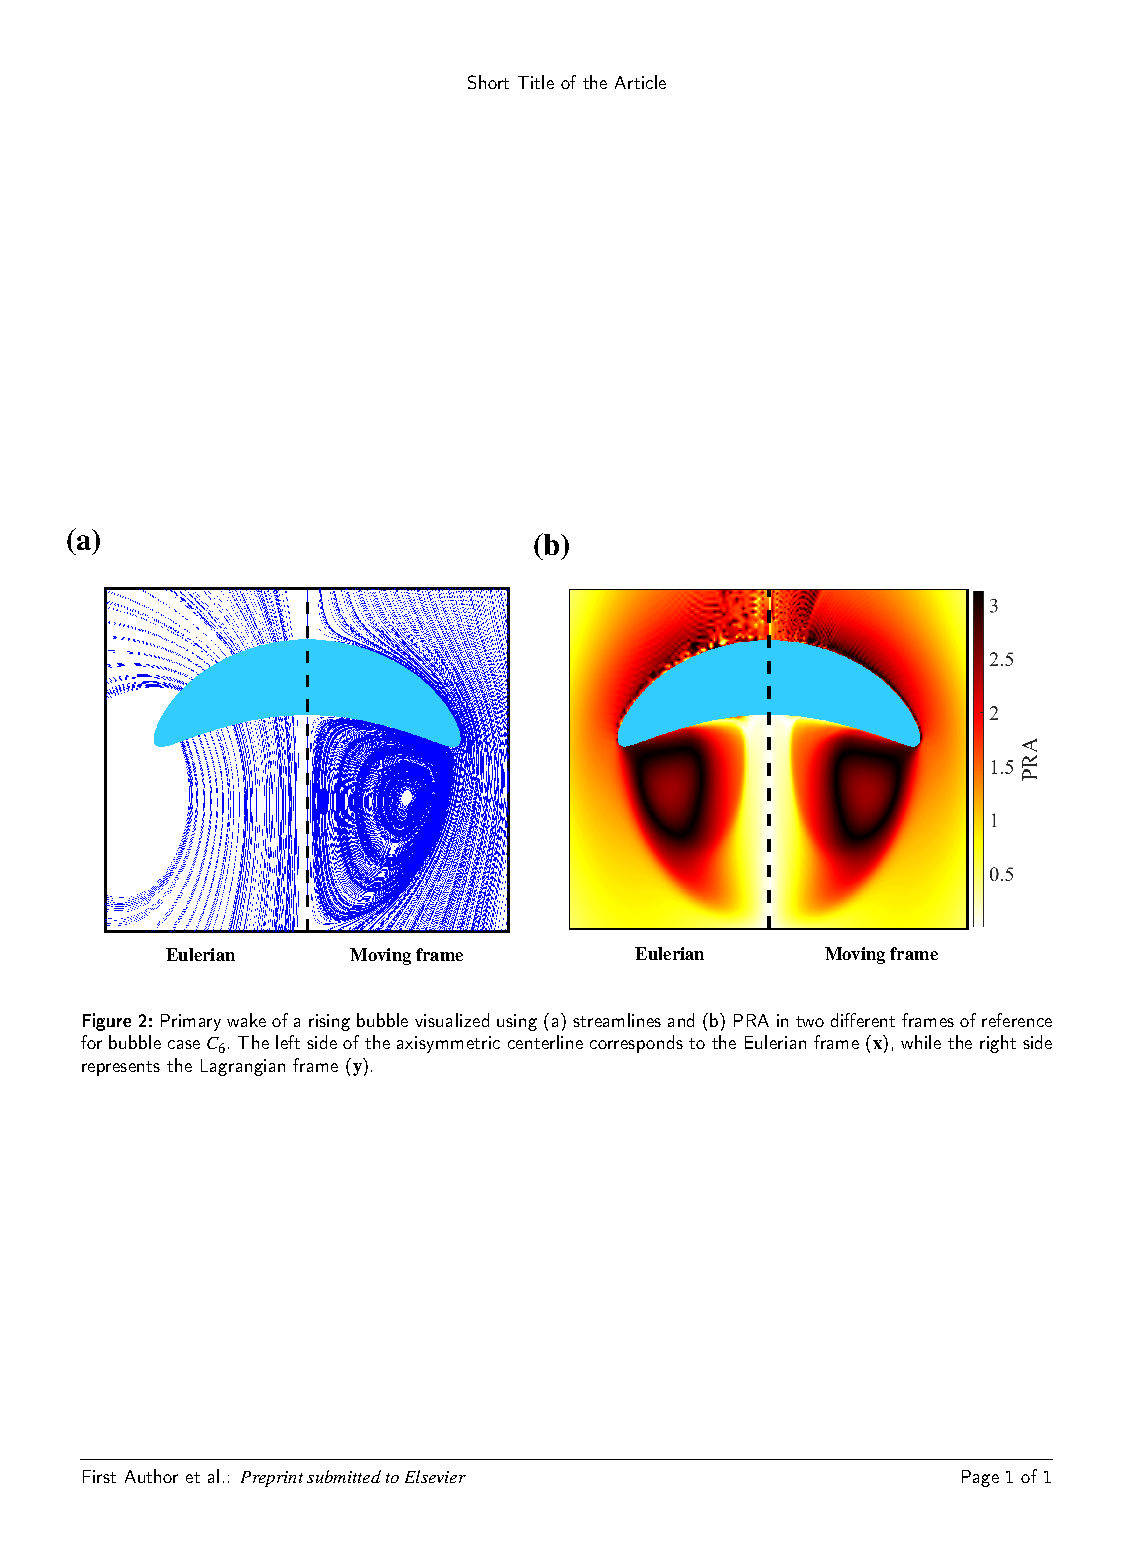
\includegraphics[scale=0.8,trim={1cm 9.5cm 1.5cm 8.5cm},clip]{Figure_2.pdf}
		\caption{Primary wake of a rising bubble visualized using (a) streamlines and (b) PRA in two different frames of reference for bubble case $C_6$. The left side of the axisymmetric centerline corresponds to the Eulerian frame ($\mathbf{x}$), while the right side represents the {\color{black}moving} frame ($\mathbf{y}$).}
		\label{Fig2}
	\end{figure}
	%%%%%%%%%%%%%%%%%%%%%%%%%%%%%________Figure_2_end___________%%%%%%%%%%%%%%%%%%%%%
	%%%%%%%%%%%%%%%%%%%%%%%%%%%%%%%%%%%%%%%%%%%%%%%%%%%%%%%%%%%%%%%%%%%%%%%%%%%%%%%%%
	%%%%%%%%%%%%%%%%%%%%%%%%%%%%%%%%%%%%%%%%%%%%%%%%%%%%%%%%%%%%%%%%%%%%%%%%%%%%%%%%%
	%%%%%%%%%%%%%%%%%%%%%%%%%%%%%%%%%%%%%%%%%%%%%%%%%%%%%%%%%%%%%%%%%%%%%%%%%%%%%%%%%
	%%%%%%%%%%%%%%%%%%%%%%%%%%%%%%%%%%%%%%%%%%%%%%%%%%%%%%%%%%%%%%%%%%%%%%%%%%%%%%%%%
	%%%%%%%%%%%%%%%%%%%%%%%%%%%%%%%%%%%%%%%%%%%%%%%%%%%%%%%%%%%%%%%%%%%%%%%%%%%%%%%%%
	
	\subsection{Different observation windows}
	\label{Different observation windows}
	
	Because of the upward translational motion of the bubble, LCSs computed over different time intervals and within different observation windows yield different structures, except for those features with steady flow characteristics such as the quasi-stationary toroidal vortices. To distinguish the structures obtained at different observation windows, the rising domain is divided into four sections denoted as I-IV as shown in Figure~\ref{Fig3}. Considering the entire rise process, the backward FTLE field, denoted as bFTLE hereafter, for $\Delta\tau_{1-3}$, is presented in Figure~\ref{Fig3}(a). In this figure, the toroidal vortices are captured just below the bubble surface at $\tau_3$, with their boundaries and the core delineated by large and small FTLE values, respectively. Downstream, however, the far-wake zone extends with low FTLE values without forming a well-defined enclosed region. Moreover, an entrainment tail characterized by large FTLE values extends along the bubble’s rise path toward region I. 
	
	To analyze the temporal evolution of the structures observed during the rise within $\Delta\tau_{1-3}$ , shorter time intervals of equal size are also analyzed, and the results are shown in Figures~\ref{Fig3}(b–d) for $\Delta\tau_{1-2}$, $\Delta\tau_{2-3}$, and $\Delta\tau_{3-4}$, respectively. Considering $\Delta\tau_{1-2}$ shown in Figure~\ref{Fig3}(b), no distinct structure is observed in regions III and IV because the fluid is stagnant and the bubble has not entered those regions yet. In region II, a toroidal vortex similar to that observed for $\Delta\tau_{1-3}$ is identified, albeit with minor structural differences. For example, the toroidal vortices extracted for $\Delta\tau_{1-2}$ are shorter in length compared to those at $\tau_{3}$ in panel (a). Additionally, the entrainment tail in region I appears wider and more pronounced compared to those observed for $\Delta\tau_{1-3}$. Such discrepancies might be attributed to the different time intervals ($\Delta\tau_{1-3}$ and $\Delta\tau_{1-2}$) and time instances ($\tau_2$ and $\tau_3$) at which the structures are extracted, highlighting the early and late stages of vortex development. In the second time interval $\Delta\tau_{2-3}$, the structures in regions III and IV correspond to those in I–II for $\Delta\tau_{1-2}$. Advancing to the time interval $\Delta\tau_{3-4}$, one can notice a similar wake structure in regions I–IV as shown in Figure~\ref{Fig3}(d). Furthermore, one may observe the decaying wake farther downstream of the bubble, with decreasing values of FTLE in regions I–II. More precisely, the structures in regions I–II for $\Delta\tau_{2-3}$ are attenuated for $\Delta\tau_{3-4}$. As the time window is shifted to late times, i.e., $\tau_{3}, \tau_{4} \rightarrow \infty$ with $\Delta\tau$ fixed, the FTLE values are expected to approach zero, suggesting the recovery of the wake toward the freestream.
	
	Considering the above observations, the wake structure of a single bubble can be characterized from LCS perspective as a primary wake including the toroidal vortices and the entrainment tails that are advected with the bubble, followed by a secondary wake with a gradual attenuation toward the freestream. The primary wake is central to mixing and transport of species. In three-phase fluidized systems, for example, the toroidal vortex and the entrainment tails could be perfect candidates for carrying solids from the bed floor to the upper regions of the column. The secondary wake, on the other hand, is recognized as a mechanism influencing the coalescence of in-line rising bubbles. For instance, the acceleration of the trailing bubble due to the wake of the leading bubble is affected by the inter-spacing $S$. In particular, higher acceleration is closely associated with stronger attraction and higher bFTLE values at shorter distances from the leading bubble. Motivated by these roles, section~\ref{transport} considers the importance of primary wake in the transport of non-inertial particles from LCS point of view whereas the secondary wake and its impact on the coalescence of two in-line rising bubbles will be investigated in section~\ref{LCS and coalescence}. 
	
	%%%%%%%%%%%%%%%%%%%%%%%%%%%%%%%%%%%%%%%%%%%%%%%%%%%%%%%%%%%%%%%%%%%%%%%%%%%%%%%%%
	%%%%%%%%%%%%%%%%%%%%%%%%%%%%%%%%%%%%%%%%%%%%%%%%%%%%%%%%%%%%%%%%%%%%%%%%%%%%%%%%%
	%%%%%%%%%%%%%%%%%%%%%%%%%%%%%%%%%%%%%%%%%%%%%%%%%%%%%%%%%%%%%%%%%%%%%%%%%%%%%%%%%
	%%%%%%%%%%%%%%%%%%%%%%%%%%%%%%%%%%%%%%%%%%%%%%%%%%%%%%%%%%%%%%%%%%%%%%%%%%%%%%%%%
	%%%%%%%%%%%%%%%%%%%%%%%%%%%%%%%%%%%%%%%%%%%%%%%%%%%%%%%%%%%%%%%%%%%%%%%%%%%%%%%%%
	%%%%%%%%%%%%%%%%%%%%%%%%%%%%%%%%%%%%%%%%%%%%%%%%%%%%%%%%%%%%%%%%%%%%%%%%%%%%%%%%%
	%%%%%%%%%%%%%%%%%%%%%%%%%%%%%________Figure_3___________%%%%%%%%%%%%%%%%%%%%%
	\begin{figure}[!t]
		\centering
		
\includegraphics[scale=1.1,trim={1.4cm 10cm 1cm 8cm},clip]{Figure_3.pdf}
		\caption{Backward FTLE fields of the rising bubble case $C_6$ (a) over the full interval $\Delta\tau_{1-3} = 4 - 20$, with observation windows indicated as I–IV. Temporal evolution of the FTLE fields within these windows, resolved into three equal sub-intervals: (b) $\Delta\tau_{1-2} = 4 - 8$ and (c) $\Delta\tau_{2-3} = 12 - 20$ , and (d) $\Delta\tau_{3-4} = 20 - 28$, showing the temporal evolution of the FTLE field.}
		\label{Fig3}
	\end{figure}
	%%%%%%%%%%%%%%%%%%%%%%%%%%%%%________Figure_3_end___________%%%%%%%%%%%%%%%%%%%%%
	%%%%%%%%%%%%%%%%%%%%%%%%%%%%%%%%%%%%%%%%%%%%%%%%%%%%%%%%%%%%%%%%%%%%%%%%%%%%%%%%%
	%%%%%%%%%%%%%%%%%%%%%%%%%%%%%%%%%%%%%%%%%%%%%%%%%%%%%%%%%%%%%%%%%%%%%%%%%%%%%%%%%
	%%%%%%%%%%%%%%%%%%%%%%%%%%%%%%%%%%%%%%%%%%%%%%%%%%%%%%%%%%%%%%%%%%%%%%%%%%%%%%%%%
	%%%%%%%%%%%%%%%%%%%%%%%%%%%%%%%%%%%%%%%%%%%%%%%%%%%%%%%%%%%%%%%%%%%%%%%%%%%%%%%%%
	%%%%%%%%%%%%%%%%%%%%%%%%%%%%%%%%%%%%%%%%%%%%%%%%%%%%%%%%%%%%%%%%%%%%%%%%%%%%%%%%%
	
	\subsection{Primary wake and transport of passive tracers}
	\label{transport}
	
	Extracting the elliptic and hyperbolic LCSs segregates the flow around the bubble into regions that evolve coherently over a specified time interval. Building on this characteristic, this section aims to identify the wake boundary and to investigate how fluid particles are transported inside and outside the wake. The analysis begins by computing the PRA and FTLE fields to extract the elliptic and hyperbolic LCSs that define the coherent flow structures. Subsequently, the wake boundary is identified, and the enclosed regions are temporally advected to examine how they govern the evolution of the wake and the transport behavior of tracers.
	
	Figure~\ref{Fig4} shows the primary wake using PRA and forward FTLE over a time interval of $\Delta\tau = 10$ at two time instances, $\tau = 3.1$ and $\tau = {\color{black}14.3}$, representing the early and late states of the wake. In general, the flow structures of the primary wake observed in the PRA field, shown in Figure~\ref{Fig4}(a,b), resemble those in the corresponding FTLE field in Figure~\ref{Fig4}(c,d). However, in the PRA field, the vortices are more pronounced and easier to detect. The overall geometry of the primary wake, characterized by the toroidal vortices, defines an oval-shaped outer boundary enclosing the recirculating region, which is bounded by ridges of the FTLE field. As seen in Figure~\ref{Fig4}(a,b), the toroidal vortices are identified as nested families of elliptic LCSs depicted as dashed lines, embraced by the outermost one shown with a solid line being the vortex boundary. It can be seen that the outermost elliptic LCS extracted at $\tau = 3.1$ in Figure~\ref{Fig4}(a), corresponding to the early formation stage of the wake, is smaller than those obtained at $\tau = {\color{black}14.3}$ in Figure~\ref{Fig4}(b). One should note that the outermost elliptic LCS may not always exhibit perfect coherence, and depending on the extraction time interval, one may or may not observe a vortex boundary with shrinking or stretching behavior at time $\tau$. In this figure, for instance, each closed elliptic LCS is associated with a stretching factor $\lambda$ varying within the range [0.82, 1.1]. The vortices tend to shrink for values of the stretching factor less than one, and no single elliptic LCS exhibits perfect coherence. In fact, the presence of an outermost elliptic LCS with a perfectly coherent loop ($\lambda = 1$) is not always guaranteed. In some time intervals, no elliptic LCSs may be observed at all, reflecting the inherent complexity and sensitivity of the extraction to $\Delta\tau$.
	
	Numerous hyperbolic LCSs are computed from the local maxima of $\lambda_2$, coinciding well with the FTLE ridges, as shown in Figures~\ref{Fig4}(c,d). An enlarged view of these structures is presented in Figure~\ref{Fig4}(e), where the outermost structure is shown in red, the innermost in blue, and the intermediate ones in green. For the given grid resolution, the outermost shrinkline is clearly identifiable, as no other lines extend outward beyond the wake region. The innermost repelling structure is selected as the last shrinkline located just before the first one circulating upward inside the bubble wake, shown in black. As one may notice, the repelling structures extend farther above the bubble, with progressively shorter extensions for the inner ones, dividing the fluid above the bubble into regions with distinct transport characteristics. In essence, each shrinkline can be thought of as a highway line that separates the fluid flow into lanes, while cross-transport is prevented from one lane to another. Hence, according to the orientation of the shrinklines above the bubble, the likelihood of fluid transport from above the bubble into the wake can be qualitatively described. For instance, fluid particles at $(0.75, 5.2)$ on the right side of the outermost shrinkline are expected to pass the bubble, whereas those at $(0.25, 5.2)$ are likely to be entrained into the wake because they lie on the side of the black line facing the bubble.
	
	%%%%%%%%%%%%%%%%%%%%%%%%%%%%%%%%%%%%%%%%%%%%%%%%%%%%%%%%%%%%%%%%%%%%%%%%%%%%%%%%%
	%%%%%%%%%%%%%%%%%%%%%%%%%%%%%%%%%%%%%%%%%%%%%%%%%%%%%%%%%%%%%%%%%%%%%%%%%%%%%%%%%
	%%%%%%%%%%%%%%%%%%%%%%%%%%%%%%%%%%%%%%%%%%%%%%%%%%%%%%%%%%%%%%%%%%%%%%%%%%%%%%%%%
	%%%%%%%%%%%%%%%%%%%%%%%%%%%%%%%%%%%%%%%%%%%%%%%%%%%%%%%%%%%%%%%%%%%%%%%%%%%%%%%%%
	%%%%%%%%%%%%%%%%%%%%%%%%%%%%%%%%%%%%%%%%%%%%%%%%%%%%%%%%%%%%%%%%%%%%%%%%%%%%%%%%%
	%%%%%%%%%%%%%%%%%%%%%%%%%%%%%%%%%%%%%%%%%%%%%%%%%%%%%%%%%%%%%%%%%%%%%%%%%%%%%%%%%
	%%%%%%%%%%%%%%%%%%%%%%%%%%%%%________Figure_4___________%%%%%%%%%%%%%%%%%%%%%
	\begin{figure}[!t]
		\centering
		
\includegraphics[scale=1.1,trim={1.4cm 11cm 1cm 8.5cm},clip]{Figure_4.pdf}
		\caption{Primary wake of a rising bubble visualized using PRA and forward FTLE fields for case $C_6$ at (a,c) $\tau = 3.1$ and (b,d) $\tau = {\color{black}14.3}$. In the PRA field, elliptic LCSs are color-coded by the stretching factor $\lambda$; the solid line denotes the outermost elliptic LCS, and the dashed lines indicate the inner ones. The FTLE contours are overlaid with the repelling structures shown as red solid lines. Panel (e) presents an enlarged view of the repelling structures at $\tau = 3.1$, used to define the wake boundary and measure the vortex length to compare it with the stagnation-based definition {\color{black}from the} velocity profile.}
		\label{Fig4}
	\end{figure}
	%%%%%%%%%%%%%%%%%%%%%%%%%%%%%________Figure_4_end___________%%%%%%%%%%%%%%%%%%%%%
	%%%%%%%%%%%%%%%%%%%%%%%%%%%%%%%%%%%%%%%%%%%%%%%%%%%%%%%%%%%%%%%%%%%%%%%%%%%%%%%%%
	%%%%%%%%%%%%%%%%%%%%%%%%%%%%%%%%%%%%%%%%%%%%%%%%%%%%%%%%%%%%%%%%%%%%%%%%%%%%%%%%%
	%%%%%%%%%%%%%%%%%%%%%%%%%%%%%%%%%%%%%%%%%%%%%%%%%%%%%%%%%%%%%%%%%%%%%%%%%%%%%%%%%
	%%%%%%%%%%%%%%%%%%%%%%%%%%%%%%%%%%%%%%%%%%%%%%%%%%%%%%%%%%%%%%%%%%%%%%%%%%%%%%%%%
	%%%%%%%%%%%%%%%%%%%%%%%%%%%%%%%%%%%%%%%%%%%%%%%%%%%%%%%%%%%%%%%%%%%%%%%%%%%%%%%%%
	
	Based on this observation, it can be hypothesized that one of the repelling structures near the wake ridge acts as the true wake boundary, effectively separating the fluid motion within the wake from the surrounding flow. In practice, the fluid on the side of this boundary facing the wake is expected to be pulled upward and entrained into the wake, such as those initiated at $(0.25, 5.2)$. To evaluate this assumption from a Lagrangian perspective, a tracer-based analysis is conducted. In this analysis, the temporal evolution of tracer particles within the regions separated by the hyperbolic LCSs are considered. The tracers are subsequently advected both forward and backward in time. The evaluation criterion for verifying a shrinkline as the wake boundary relies on the transport of fluid particles near the upper part of the bubble surface. Specifically, a shrinkline is identified as the wake boundary if the fluid particles located on the side of the shrinkline facing the bubble surface are eventually advected into the wake region. In other words, particles released from the bubble roof that end up within the recirculating region delineated by the shrinkline indicate that this structure acts as the effective wake boundary. Adopting this criterion, the innermost repelling structure (blue line)—corresponding to the one with the maximum $Z$ coordinate at $R=0$ and located just before the first repelling structure inside the wake that circulates toward the wake (black line)—can be considered the most plausible candidate for the true wake boundary. It should be noted that the black line is already inside the wake and can not be considered a true wake boundary.
	
	To further evaluate the validity of this LCS-based boundary and to compare it with previous definitions, the wake boundary length based on the stagnation point is also considered. Following this approach, the wake length $L_w$, shown in Figure~\ref{Fig4}(e), is defined as the distance between the front stagnation point of the bubble and the rear stagnation point of the wake, obtained from the velocity profile along the symmetry axis ($R=0$). These two critical points, shown as red dots in Figure~\ref{Fig4}(e), correspond to the locations where the upward velocity component equals the bubble rise velocity. In the LCS framework, the wake length is analogously measured as the distance between the front stagnation point and the $Z$-coordinate of the identified shrinkline selected as the wake boundary—here, the innermost blue shrinkline. A preliminary comparison indicates that the rear stagnation point lies close to the innermost hyperbolic LCS, with a deviation of approximately 1\%. A temporal comparison of the wake length $L_w$ during the rise is further examined in Figure~\ref{Fig6}, which will be discussed at the end of this section.  
	
	Following the procedure described previously, the outermost and innermost repelling LCSs for bubble case $C_6$ at $\tau = 3.6$ are identified and shown in Figure~\ref{Fig5}(d) as dashed red and blue lines, respectively. Owing to the material coherence and impermeability of these repelling structures to fluid transport, distinct flow regions can be identified within the wake. To analyze the evolution of these regions and to verify the validity of the shrinklines as the wake boundary, the structures are advected both forward [Figures~\ref{Fig5}(e–g)] and backward [Figures~\ref{Fig5}(a–c)] in time. During forward advection, the outermost and innermost shrinklines at $\tau = 9.2$, $14.8$, and $19.5$ are computed with the same time interval and illustrated using dash-dotted, dotted, and solid lines. The shrinklines obtained at earlier times are advected and shown with their corresponding line styles at later times. Tracer particles, color-coded according to their transport behavior (see the color bar below Figure~\ref{Fig5} marked with the associated transport behavior), are distributed within these regions. On this color bar, the light blue and purple regions at the two extremes represent particles belonging to the external flow and the vortex core, respectively, while particles in the other regions have different transport behaviors that will be discussed in the following paragraphs.
	
	%%%%%%%%%%%%%%%%%%%%%%%%%%%%%%%%%%%%%%%%%%%%%%%%%%%%%%%%%%%%%%%%%%%%%%%%%%%%%%%%%
	%%%%%%%%%%%%%%%%%%%%%%%%%%%%%%%%%%%%%%%%%%%%%%%%%%%%%%%%%%%%%%%%%%%%%%%%%%%%%%%%%
	%%%%%%%%%%%%%%%%%%%%%%%%%%%%%%%%%%%%%%%%%%%%%%%%%%%%%%%%%%%%%%%%%%%%%%%%%%%%%%%%%
	%%%%%%%%%%%%%%%%%%%%%%%%%%%%%%%%%%%%%%%%%%%%%%%%%%%%%%%%%%%%%%%%%%%%%%%%%%%%%%%%%
	%%%%%%%%%%%%%%%%%%%%%%%%%%%%%%%%%%%%%%%%%%%%%%%%%%%%%%%%%%%%%%%%%%%%%%%%%%%%%%%%%
	%%%%%%%%%%%%%%%%%%%%%%%%%%%%%%%%%%%%%%%%%%%%%%%%%%%%%%%%%%%%%%%%%%%%%%%%%%%%%%%%%
	%%%%%%%%%%%%%%%%%%%%%%%%%%%%%________Figure_5___________%%%%%%%%%%%%%%%%%%%%%
	\begin{figure}[!t]
		\centering
		
\includegraphics[scale=1.09,trim={1.4cm 10.1cm 1cm 7cm},clip]{Figure_5.pdf}
		\caption{Temporal backward [(a) $\tau = 0.05$, (b) $0.75$, (c) $2.0$] and forward [(e) $\tau = 5.4$, (f) $7.0$, (g) $8.0$] evolution of flow regions separated by hyperbolic LCSs obtained from the forward FTLE field with $\Delta\tau = 10$ at $\tau_0 = 3.6$, shown in (d), for bubble case $C_6$. The outermost and innermost repelling structures in (d) are indicated by red and blue dashed lines, respectively. In panels (e–g), the corresponding repelling structures computed at each time are shown as red and blue dash-dotted, dotted, and solid lines. The color bar below the panels indicates the transport behavior of tracers in each region.}
		\label{Fig5}
	\end{figure}
	%%%%%%%%%%%%%%%%%%%%%%%%%%%%%________Figure_5_end___________%%%%%%%%%%%%%%%%%%%%%
	%%%%%%%%%%%%%%%%%%%%%%%%%%%%%%%%%%%%%%%%%%%%%%%%%%%%%%%%%%%%%%%%%%%%%%%%%%%%%%%%%
	%%%%%%%%%%%%%%%%%%%%%%%%%%%%%%%%%%%%%%%%%%%%%%%%%%%%%%%%%%%%%%%%%%%%%%%%%%%%%%%%%
	%%%%%%%%%%%%%%%%%%%%%%%%%%%%%%%%%%%%%%%%%%%%%%%%%%%%%%%%%%%%%%%%%%%%%%%%%%%%%%%%%
	%%%%%%%%%%%%%%%%%%%%%%%%%%%%%%%%%%%%%%%%%%%%%%%%%%%%%%%%%%%%%%%%%%%%%%%%%%%%%%%%%
	%%%%%%%%%%%%%%%%%%%%%%%%%%%%%%%%%%%%%%%%%%%%%%%%%%%%%%%%%%%%%%%%%%%%%%%%%%%%%%%%%
	
	Considering the forward advection, fluid particles initialized in the the light-blue region outside the outermost shrinkline pass the bubble without significant interaction with the wake. They are coded as light-blue because they are drawn upward by the influence of the wake but ultimately remain behind and become nearly stagnant as $\tau \rightarrow \infty$. This behavior is illustrated in Figure~\ref{Fig5}(g), where the light-blue particles below the dashed red line are left behind downstream. In contrast, the forward-in-time evolution of the orange particles situated between the bubble’s top surface and the innermost shrinkline exhibits a distinct behavior. These particles are initially marked in orange because they ultimately end up in the wake (Figures~\ref{Fig5}(d,e)). Their evolution is highlighted by colors corresponding to their instantaneous transport characteristics. They enter the bubble’s wake while drawing upward (orange), move toward the vortex core (pink), and eventually begin to rotate as shown in Figures~\ref{Fig5}(e-g).
	
	Interesting transport characteristics are observed for the green tracers located within the narrow gap between the innermost and outermost shrinklines. These tracers are colored green because they exhibit transitional behavior—some are entrained upward into the wake and behave similarly to the orange particles, some remain in transition, and others gradually tend to move toward the external flow. Whether the green particles at $\tau_0$ are entrained into the wake, repelled toward the external flow, or maintain their transitional behavior is governed by the positions of the innermost and outermost shrinklines obtained at the subsequent time $\tau_1$. As shown in Figures~\ref{Fig5}(d) and (e) for $\tau_0 = 3.6$ and $\tau_1 = 9.2$, respectively, green tracers released at $\tau_0$ that lie between the innermost and outermost shrinklines at $\tau_1$ continue to exhibit transitional behavior and retain their green color. Meanwhile, tracers located on the side of the innermost shrinkline at $\tau_1$ facing the wake are entrained into the wake, gradually changing color from green to yellow, while those on the side of the outermost shrinkline facing the external flow tend to fall behind and drift outward, with their color shifting from green to blue. Through a similar process, the transport of the green tracers at $\tau_1 = 9.2$ is governed by the shrinklines obtained at $\tau_2 = 14.8$, and subsequently, the transport of green tracers at $\tau_3$ is governed by those at $\tau_3 = 19.5$. This analysis highlights the critical role of the shrinkines in entrainment or escape of the tracers initially released at $\tau_0$ above the bubble's surface.
	
	In addition, the above tracers-based analysis shows that the innermost shrinkline can be considered as a true wake boundary due to the fact that tracers on the wake-facing side of these lines computed at each time are consistently entrained into the wake. Moreover, another supporting fact in this regard is the increasing length of the wake measured from the $Z$ component of the innermost shrinkline at $R = 0$ with time as shown in Figures~\ref{Fig5}(d-f). As can be seen, the length of the wake {\color{black}is} estimated to be $1.4$, $1.9$, and $2.1$, at $\tau=3.6$, $9.2$ and $14.8$, respectively. However, the {\color{black}length} of wake reaches a constant value suggesting the full development of the wake. These {\color{black}observations} are in agreement with previous experimental results of \citet{fan1986} reporting the same wake characteristics. 
	
	The temporal variation of the wake length measured using LCS is compared with that based on the stagnation points, and the results are shown in Figure~\ref{Fig6}(a) together with other rise characteristics, including the Reynolds number and the circularity profile. It is interesting to note that, even though the rise velocity reaches a steady state at around $\tau=5$ and the bubble ceases to deform at $\tau = 10$, the wake length continues to increase for both the stagnation- and LCS-based measurements. As shown, the stagnation-based wake length is slightly underestimated compared to the LCS-based one, although both eventually converge to an identical steady-state value. The stabilized length of the primary wake is measured for seven different cases using the innermost shrinkline and compared with the experimental correlation of \citet{Bhaga1980Exp}, as shown in Figure~\ref{Fig6}(b). A good agreement is observed across a wide range of Morton numbers. Furthermore, \citet{Monica2016} demonstrated that a critical Reynolds number exists as a function of the Bond number, below which toroidal vortices do not form. This is confirmed for case $C_4$ with $Bo = 22$, where $Re < Re_c$ and no closed toroidal vortices are detected. This consistency check highlights the robustness of the LCS-based approach in identifying coherent flow structures across different flow configurations.
	
	
	%%%%%%%%%%%%%%%%%%%%%%%%%%%%%%%%%%%%%%%%%%%%%%%%%%%%%%%%%%%%%%%%%%%%%%%%%%%%%%%%%
	%%%%%%%%%%%%%%%%%%%%%%%%%%%%%%%%%%%%%%%%%%%%%%%%%%%%%%%%%%%%%%%%%%%%%%%%%%%%%%%%%
	%%%%%%%%%%%%%%%%%%%%%%%%%%%%%%%%%%%%%%%%%%%%%%%%%%%%%%%%%%%%%%%%%%%%%%%%%%%%%%%%%
	%%%%%%%%%%%%%%%%%%%%%%%%%%%%%%%%%%%%%%%%%%%%%%%%%%%%%%%%%%%%%%%%%%%%%%%%%%%%%%%%%
	%%%%%%%%%%%%%%%%%%%%%%%%%%%%%%%%%%%%%%%%%%%%%%%%%%%%%%%%%%%%%%%%%%%%%%%%%%%%%%%%%
	%%%%%%%%%%%%%%%%%%%%%%%%%%%%%%%%%%%%%%%%%%%%%%%%%%%%%%%%%%%%%%%%%%%%%%%%%%%%%%%%%
	%%%%%%%%%%%%%%%%%%%%%%%%%%%%%________Figure_6___________%%%%%%%%%%%%%%%%%%%%%
	\begin{figure}[!t]
		\centering
		
\includegraphics[scale=1.1,trim={1.4cm 11cm 1cm 7cm},clip]{Figure_6.pdf}
		\caption{(a) Temporal evolution of the Reynolds number, circularity, and wake length $L_w$ measured using the stagnation-point and LCS-based definitions. (b) Stabilized wake length obtained from LCS analysis compared with the experimental correlation of~\color{black}{\citet{Bhaga1980Exp}} for the bubble cases listed in Table~\ref{Table1}.}
		\label{Fig6}
	\end{figure}
	%%%%%%%%%%%%%%%%%%%%%%%%%%%%%________Figure_6_end___________%%%%%%%%%%%%%%%%%%%%%
	%%%%%%%%%%%%%%%%%%%%%%%%%%%%%%%%%%%%%%%%%%%%%%%%%%%%%%%%%%%%%%%%%%%%%%%%%%%%%%%%%
	%%%%%%%%%%%%%%%%%%%%%%%%%%%%%%%%%%%%%%%%%%%%%%%%%%%%%%%%%%%%%%%%%%%%%%%%%%%%%%%%%
	%%%%%%%%%%%%%%%%%%%%%%%%%%%%%%%%%%%%%%%%%%%%%%%%%%%%%%%%%%%%%%%%%%%%%%%%%%%%%%%%%
	%%%%%%%%%%%%%%%%%%%%%%%%%%%%%%%%%%%%%%%%%%%%%%%%%%%%%%%%%%%%%%%%%%%%%%%%%%%%%%%%%
	%%%%%%%%%%%%%%%%%%%%%%%%%%%%%%%%%%%%%%%%%%%%%%%%%%%%%%%%%%%%%%%%%%%%%%%%%%%%%%%%%
	
	
	\subsection{Secondary wake and bubble coalescence}
	\label{LCS and coalescence}
	Bubble coalescence is a complex phenomenon that varies significantly depending on several parameters. These include the initial configuration of the bubbles and their inter-spacing during the rise, the size of the leading bubble, its terminal shape and corresponding wake, and the prevailing flow regime. Generally, coalescence consists of three stages: acceleration of the trailing bubble, its penetration into the near-wake of the leading bubble, and, finally, drainage of the intervening liquid film leading to merger. The analysis in the present work is limited to the acceleration phase, which acts as the primary trigger for coalescence. The effects of two important varying parameters—namely, the inter-spacing $S$ and the size of the leading bubble represented by the Reynolds number ($Re$)—are investigated in this study.

	%%%%%%%%%%%%%%%%%%%%%%%%%%%%%%%%%%%%%%%%%%%%%%%%%%%%%%%%%%%%%%%%%%%%%%%%%%%%%%%%%
	%%%%%%%%%%%%%%%%%%%%%%%%%%%%%%%%%%%%%%%%%%%%%%%%%%%%%%%%%%%%%%%%%%%%%%%%%%%%%%%%%
	%%%%%%%%%%%%%%%%%%%%%%%%%%%%%%%%%%%%%%%%%%%%%%%%%%%%%%%%%%%%%%%%%%%%%%%%%%%%%%%%%
	%%%%%%%%%%%%%%%%%%%%%%%%%%%%%%%%%%%%%%%%%%%%%%%%%%%%%%%%%%%%%%%%%%%%%%%%%%%%%%%%%
	%%%%%%%%%%%%%%%%%%%%%%%%%%%%%%%%%%%%%%%%%%%%%%%%%%%%%%%%%%%%%%%%%%%%%%%%%%%%%%%%%
	%%%%%%%%%%%%%%%%%%%%%%%%%%%%%%%%%%%%%%%%%%%%%%%%%%%%%%%%%%%%%%%%%%%%%%%%%%%%%%%%%
	%%%%%%%%%%%%%%%%%%%%%%%%%%%%%________Figure_6___________%%%%%%%%%%%%%%%%%%%%%
	\begin{figure}[!t]
		\centering
		
\includegraphics[scale=1.1,trim={1.4cm 11.5cm 1cm 9.3cm},clip]{Figure_7.pdf}
		\caption{Backward FTLE fields with $\Delta \tau = 2.5$ for rising bubble cases $C_4$ ($\mathrm{Re} = 18.3$) and $C_7$ ($\mathrm{Re} = 61$) at different separation distances. Panels (a) and (b) correspond to case $C_4$ with $S = 6$ and $S = 9$, respectively, while panels (c) and (d) correspond to case $C_7$ with $S = 6$ and $S = 9$. Panel (e) shows the acceleration of the trailing bubble case $C_4$ behind the leading bubble over the same time interval $\Delta \tau = 2.5$, measured at the same vertical location where the bFTLE fields are evaluated.}
		\label{Fig7}
	\end{figure}
	%%%%%%%%%%%%%%%%%%%%%%%%%%%%%________Figure_6_end___________%%%%%%%%%%%%%%%%%%%%%
	%%%%%%%%%%%%%%%%%%%%%%%%%%%%%%%%%%%%%%%%%%%%%%%%%%%%%%%%%%%%%%%%%%%%%%%%%%%%%%%%%
	%%%%%%%%%%%%%%%%%%%%%%%%%%%%%%%%%%%%%%%%%%%%%%%%%%%%%%%%%%%%%%%%%%%%%%%%%%%%%%%%%
	%%%%%%%%%%%%%%%%%%%%%%%%%%%%%%%%%%%%%%%%%%%%%%%%%%%%%%%%%%%%%%%%%%%%%%%%%%%%%%%%%
	%%%%%%%%%%%%%%%%%%%%%%%%%%%%%%%%%%%%%%%%%%%%%%%%%%%%%%%%%%%%%%%%%%%%%%%%%%%%%%%%%
	%%%%%%%%%%%%%%%%%%%%%%%%%%%%%%%%%%%%%%%%%%%%%%%%%%%%%%%%%%%%%%%%%%%%%%%%%%%%%%%%%
	
	The presence of the trailing bubble alters the flow field behind the leading bubble, making it highly complex to study the secondary wake effects of the leading bubble during the acceleration phase. Hence, the LCS analysis is performed in the absence of the trailing bubble, considering a single leading-bubble rise, which is later used to interpret the actual two-bubble scenario through the measured rise velocities. {\color{black}In this study, attraction regions are first diagnosed from \textit{single-bubble} bFTLE fields in a fixed window; we then validate the predicted trends in separate \textit{inline, axisymmetric} two-bubble simulations by measuring the trailing-bubble velocity deficit (Fig.~\ref{Fig7}e).} This configuration enables assessment of how the flow field generated by the leading bubble influences a trailing bubble positioned at a given distance, thereby demonstrating the ability of the bFTLE field to capture and explain the trailing-bubble acceleration mechanism. Following this strategy, the analysis considers the bFTLE fields computed over a time interval of $\Delta\tau = \tau_1 - \tau_0 = 2.5$ within a fixed rectangular observation window defined as $Z = 12.5$–$15.5$ and $R = 0$–$4$, as shown in Figure~\ref{Fig7}(a,b) and (c,d) for the leading-bubble cases $C_4$ and $C_7$ with rising Reynolds number of $18.3$ and 61, respectively. Panels (a) and (c) correspond to the bFTLE fields obtained at $\tau_1$ and the inter-spacing distance between the assumed positions of the bubbles at $\tau_0$ is initially $S = 6$, while panels (b) and (d) correspond to $S = 9$. It should be emphasized that these bFTLE fields are computed for a single leading-bubble rise; the trailing bubble is not physically present in the simulation but is hypothetically assumed to have its upper surface located at $Z = 12.5$, marking the entry of the observation window, at $\tau_0$. 
	
	The overall assessment of the bFTLE fields reveals regions of stronger attraction in forward time for the larger bubble case $C_7$ compared to $C_4$ at the same inter-spacing, as shown in Figures~\ref{Fig7}(c,d) and (a,b), respectively. It may be inferred that if the trailing bubble $C_4$ at time $\tau_0$ were positioned at $Z = 12.5$ and rose behind the larger bubble $C_7$, it would be subjected to stronger wake effects and therefore accelerate more than if it rose behind the bubble $C_4$ within the same inter-spacing. Similarly, it can be shown that increasing the inter-spacing between the bubbles will weaken the attraction in forward time as shown for bubble case $C_7$ for inter-spacings $S=6$ and $S=9$ in Figures~\ref{Fig7}(c) and (a), respectively. 
	
	These observations are supported by the velocity deficit measurements of the actual two-bubble rise setup. In this configuration, the acceleration of the trailing bubble for the same setups as those assumed in panels (a–d) is measured through the velocity deficit of the trailing bubble. Blue and red solid lines correspond to configurations of panels (a) and (c) for inter-spacing of $S=6$ while the dashed lines correspond to the same bubbles for inter-spacing of $S=9$. During the same time interval $\Delta\tau$ at which the FTLE fields are computed, the velocity deficit of the trailing bubble is measured as $V_{TR} - V_{TR_0}$, where $V_{TR_0}$ is the velocity at $Z = 12.5$, normalized by the rise velocity $V_s$ of the trailing bubble in the single-rise configuration (i.e., without a leading bubble upstream). As can be seen, the trailing bubble rising behind the larger bubble case $C_7$ gains more velocity than in case $C_4$, reflecting the influence of the Reynolds number and the stronger attraction regions revealed by the bFTLE fields corresponding to panels (a) and (c). Meanwhile, the trailing bubble gains less velocity when the inter-spacing is increased from $S = 6$ to $S = 9$, as shown by the red solid and dashed lines for the leading-bubble case $C_7$ corresponding to panels (c) and (d), where the FTLE values are weakened. Finally, one may notice that regardless of the inter-spacing of the bubbles, the acceleration is not considerable for the leading bubble case $C_4$ compared to the larger bubble as the blue dashed and solid lines represent small rise velocity deficit values. 
	
	\section{Concluding remarks}
	\label{Concluding remarks}
	
	This work demonstrates that Lagrangian Coherent Structures provide a robust and objective framework for characterizing the wake dynamics of a single rising bubble {\color{black}in laminar, inline (axisymmetric) configurations}. Here, we clearly demonstrate the pitfalls and misleading consequences of employing non-objective flow structure characterization (by pointing to a streamline example). The primary wake is identified as a material region enclosed by repelling structures that act as effective transport barriers. The innermost repelling LCS extracted from the FTLE field {\color{black}agrees} with a stagnation-based wake-length metric and matches the trend of the {\color{black}Bhaga \& Weber} correlation. The temporal evolution of this boundary reveals the gradual development and stabilization of the toroidal vortices, in agreement with previous experimental correlations.
	
	The analysis of tracer transport shows that particles released above the bubble are either entrained into the wake, remain in transitional regions, or are repelled outward depending on their initial position relative to the repelling structures. This provides a clear material description of mass-exchange processes around the bubble. The LCS analysis further clarifies the acceleration mechanism of a trailing bubble, where stronger attracting regions in the backward-time FTLE field correspond to enhanced wake influence and increased velocity deficit, qualitatively explaining the observed rise acceleration in two-bubble systems. Although this qualitative agreement establishes a clear physical link between wake topology and bubble interaction, the present LCS analysis does not yield a quantitative correlation between FTLE magnitude and the rise velocity; such connection would require coupling the LCS framework with detailed force-balance modeling, which is beyond the present scope.
	
	Overall, the study demonstrates that the LCS-based approach unifies wake characterization, tracer transport, and inter-bubble interaction within a single material-coherent framework, offering new insight into the dynamics of buoyancy-driven multiphase flows.
	\\
	\\
	%---------------------------------
	{\noindent \bf{Funding}} \\	
	The work was supported by the Research Council of Norway (NRC) (Grant no. 334652). \\
	\\
	{\bf{Conflict of interest}} \\
	The authors declare no conflict of interest. \\
	\\
	{\bf{Data availability}} \\
	%--------------------------------------
	The data that support the findings of this study are available from the corresponding author upon reasonable request. \\
	
	\nolinenumbers % <-- Stop line numbering
	
	\section*{References}
	
	\bibliography{libraryLCS}
	
\end{document}
%
% ****** End of file  ******
